% GNUPLOT: LaTeX picture with Postscript
\begingroup
  \makeatletter
  \providecommand\color[2][]{%
    \GenericError{(gnuplot) \space\space\space\@spaces}{%
      Package color not loaded in conjunction with
      terminal option `colourtext'%
    }{See the gnuplot documentation for explanation.%
    }{Either use 'blacktext' in gnuplot or load the package
      color.sty in LaTeX.}%
    \renewcommand\color[2][]{}%
  }%
  \providecommand\includegraphics[2][]{%
    \GenericError{(gnuplot) \space\space\space\@spaces}{%
      Package graphicx or graphics not loaded%
    }{See the gnuplot documentation for explanation.%
    }{The gnuplot epslatex terminal needs graphicx.sty or graphics.sty.}%
    \renewcommand\includegraphics[2][]{}%
  }%
  \providecommand\rotatebox[2]{#2}%
  \@ifundefined{ifGPcolor}{%
    \newif\ifGPcolor
    \GPcolortrue
  }{}%
  \@ifundefined{ifGPblacktext}{%
    \newif\ifGPblacktext
    \GPblacktexttrue
  }{}%
  % define a \g@addto@macro without @ in the name:
  \let\gplgaddtomacro\g@addto@macro
  % define empty templates for all commands taking text:
  \gdef\gplbacktext{}%
  \gdef\gplfronttext{}%
  \makeatother
  \ifGPblacktext
    % no textcolor at all
    \def\colorrgb#1{}%
    \def\colorgray#1{}%
  \else
    % gray or color?
    \ifGPcolor
      \def\colorrgb#1{\color[rgb]{#1}}%
      \def\colorgray#1{\color[gray]{#1}}%
      \expandafter\def\csname LTw\endcsname{\color{white}}%
      \expandafter\def\csname LTb\endcsname{\color{black}}%
      \expandafter\def\csname LTa\endcsname{\color{black}}%
      \expandafter\def\csname LT0\endcsname{\color[rgb]{1,0,0}}%
      \expandafter\def\csname LT1\endcsname{\color[rgb]{0,1,0}}%
      \expandafter\def\csname LT2\endcsname{\color[rgb]{0,0,1}}%
      \expandafter\def\csname LT3\endcsname{\color[rgb]{1,0,1}}%
      \expandafter\def\csname LT4\endcsname{\color[rgb]{0,1,1}}%
      \expandafter\def\csname LT5\endcsname{\color[rgb]{1,1,0}}%
      \expandafter\def\csname LT6\endcsname{\color[rgb]{0,0,0}}%
      \expandafter\def\csname LT7\endcsname{\color[rgb]{1,0.3,0}}%
      \expandafter\def\csname LT8\endcsname{\color[rgb]{0.5,0.5,0.5}}%
    \else
      % gray
      \def\colorrgb#1{\color{black}}%
      \def\colorgray#1{\color[gray]{#1}}%
      \expandafter\def\csname LTw\endcsname{\color{white}}%
      \expandafter\def\csname LTb\endcsname{\color{black}}%
      \expandafter\def\csname LTa\endcsname{\color{black}}%
      \expandafter\def\csname LT0\endcsname{\color{black}}%
      \expandafter\def\csname LT1\endcsname{\color{black}}%
      \expandafter\def\csname LT2\endcsname{\color{black}}%
      \expandafter\def\csname LT3\endcsname{\color{black}}%
      \expandafter\def\csname LT4\endcsname{\color{black}}%
      \expandafter\def\csname LT5\endcsname{\color{black}}%
      \expandafter\def\csname LT6\endcsname{\color{black}}%
      \expandafter\def\csname LT7\endcsname{\color{black}}%
      \expandafter\def\csname LT8\endcsname{\color{black}}%
    \fi
  \fi
    \setlength{\unitlength}{0.0500bp}%
    \ifx\gptboxheight\undefined%
      \newlength{\gptboxheight}%
      \newlength{\gptboxwidth}%
      \newsavebox{\gptboxtext}%
    \fi%
    \setlength{\fboxrule}{0.5pt}%
    \setlength{\fboxsep}{1pt}%
\begin{picture}(10080.00,6480.00)%
    \gplgaddtomacro\gplbacktext{%
      \csname LTb\endcsname%%
      \put(946,704){\makebox(0,0)[r]{\strut{}$-160$}}%
      \put(946,1272){\makebox(0,0)[r]{\strut{}$-140$}}%
      \put(946,1841){\makebox(0,0)[r]{\strut{}$-120$}}%
      \put(946,2409){\makebox(0,0)[r]{\strut{}$-100$}}%
      \put(946,2977){\makebox(0,0)[r]{\strut{}$-80$}}%
      \put(946,3546){\makebox(0,0)[r]{\strut{}$-60$}}%
      \put(946,4114){\makebox(0,0)[r]{\strut{}$-40$}}%
      \put(946,4682){\makebox(0,0)[r]{\strut{}$-20$}}%
      \put(946,5251){\makebox(0,0)[r]{\strut{}$0$}}%
      \put(946,5819){\makebox(0,0)[r]{\strut{}$20$}}%
      \put(1078,484){\makebox(0,0){\strut{}$0$}}%
      \put(2307,484){\makebox(0,0){\strut{}$0,02$}}%
      \put(3537,484){\makebox(0,0){\strut{}$0,04$}}%
      \put(4766,484){\makebox(0,0){\strut{}$0,06$}}%
      \put(5995,484){\makebox(0,0){\strut{}$0,08$}}%
      \put(7224,484){\makebox(0,0){\strut{}$0,1$}}%
      \put(8454,484){\makebox(0,0){\strut{}$0,12$}}%
      \put(9683,484){\makebox(0,0){\strut{}$0,14$}}%
    }%
    \gplgaddtomacro\gplfronttext{%
      \csname LTb\endcsname%%
      \put(209,3261){\rotatebox{-270}{\makebox(0,0){\strut{}Vertikale Position $y/\si{\milli\meter}$}}}%
      \put(5380,154){\makebox(0,0){\strut{}Zeit $t/\si{\second}$}}%
      \csname LTb\endcsname%%
      \put(5465,5646){\makebox(0,0)[r]{\strut{}Kugel 1}}%
      \csname LTb\endcsname%%
      \put(5465,5426){\makebox(0,0)[r]{\strut{}Kugel 2}}%
      \csname LTb\endcsname%%
      \put(5465,5206){\makebox(0,0)[r]{\strut{}Kugel 3}}%
      \csname LTb\endcsname%%
      \put(5465,4986){\makebox(0,0)[r]{\strut{}Kugel 4}}%
      \csname LTb\endcsname%%
      \put(5465,4766){\makebox(0,0)[r]{\strut{}Kugel 5}}%
      \csname LTb\endcsname%%
      \put(5465,4546){\makebox(0,0)[r]{\strut{}Kugel 6}}%
      \csname LTb\endcsname%%
      \put(5465,4326){\makebox(0,0)[r]{\strut{}Kugel 7}}%
      \csname LTb\endcsname%%
      \put(5465,4106){\makebox(0,0)[r]{\strut{}Kugel 8}}%
      \csname LTb\endcsname%%
      \put(5465,3886){\makebox(0,0)[r]{\strut{}Kugel 9}}%
      \csname LTb\endcsname%%
      \put(8696,5646){\makebox(0,0)[r]{\strut{}$-1039,02016t + (0,97689)$}}%
      \csname LTb\endcsname%%
      \put(8696,5426){\makebox(0,0)[r]{\strut{}$-1097,64782t + (0,28449)$}}%
      \csname LTb\endcsname%%
      \put(8696,5206){\makebox(0,0)[r]{\strut{}$-1155,39617t + (-0,01640)$}}%
      \csname LTb\endcsname%%
      \put(8696,4986){\makebox(0,0)[r]{\strut{}$-1082,00957t + (0,86551)$}}%
      \csname LTb\endcsname%%
      \put(8696,4766){\makebox(0,0)[r]{\strut{}$-1140,03598t + (0,72630)$}}%
      \csname LTb\endcsname%%
      \put(8696,4546){\makebox(0,0)[r]{\strut{}$-1139,65074t + (0,44495)$}}%
      \csname LTb\endcsname%%
      \put(8696,4326){\makebox(0,0)[r]{\strut{}$-1116,62708t + (0,82640)$}}%
      \csname LTb\endcsname%%
      \put(8696,4106){\makebox(0,0)[r]{\strut{}$-1125,03549t + (0,75324)$}}%
      \csname LTb\endcsname%%
      \put(8696,3886){\makebox(0,0)[r]{\strut{}$-1091,94893t + (1,08144)$}}%
      \csname LTb\endcsname%%
      \put(5380,6149){\makebox(0,0){\strut{}Fallverlauf der Stahlkugeln}}%
    }%
    \gplbacktext
    \put(0,0){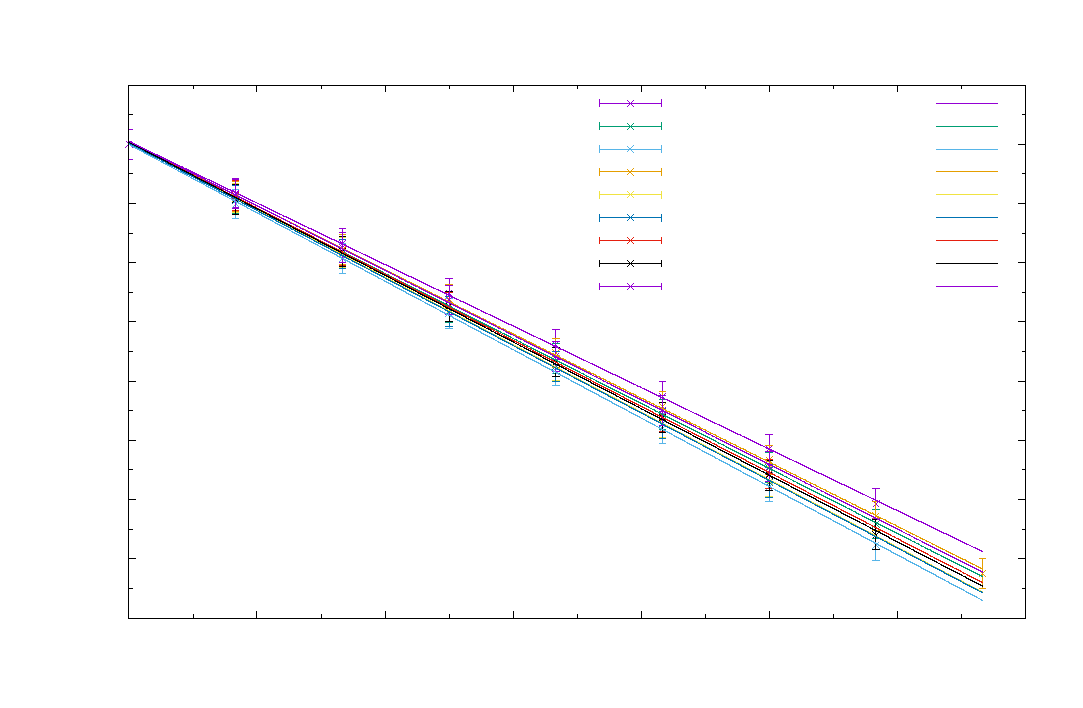
\includegraphics[width={504.00bp},height={324.00bp}]{tv2-plot}}%
    \gplfronttext
  \end{picture}%
\endgroup
